One more considered approach how to recognize an issue's topic was using the GIT labels. Labels on GitHub help you organize and prioritize your work. You can apply labels to issues and pull requests to signify priority, category, or any other information you find useful. There are two types of labels - default and custom. GitHub provides default ones in every new repository. All default labels can be seen in table \ref{fig:defaultLabels} and can be used to create a standard workflow in a repository:

\begin{figure}[H]%
    \centering
	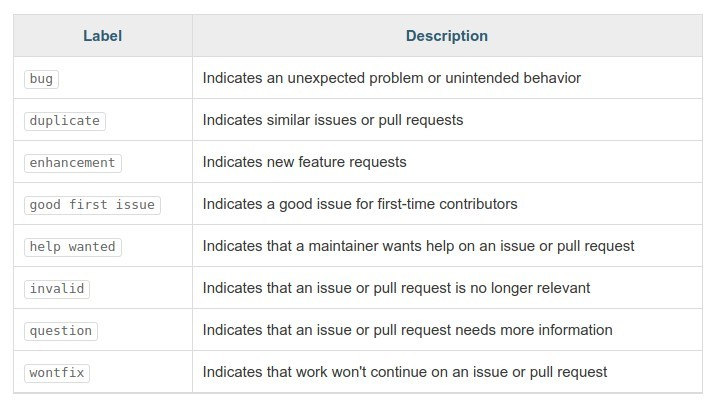
\includegraphics[width=8cm]{defaultLabels.jpg}
    \caption{Default Git labels provided for every repository}%
    \label{fig:defaultLabels}%
\end{figure}

These default labels come as a big help in directing the project and targeting the most important issues, but they don't say much about the nature of the issue itself.

The custom tags tell are used to specify the part of the project, where the issue is located but they still don't give any semantic information about the issue itself. That's the reason why this approach was rejected. 
